\documentclass{article}

\usepackage[a4paper, portrait, margin=1.5cm]{geometry}

\usepackage{fancyhdr}
\usepackage{hyperref}
\setlength{\headheight}{15pt}

\usepackage[table]{xcolor}
%\usepackage{minipage}
\usepackage{float}
\usepackage{svg}
\usepackage{ltablex}

\setlength{\arrayrulewidth}{0.2mm}

\usepackage{tikz}
\usetikzlibrary{shapes, arrows.meta, positioning}

\usepackage{textcomp}
\usepackage{amsmath}
\usepackage{amsfonts}
\usepackage{amssymb}
\usepackage{mathrsfs}
\usepackage{mathtools}
\usepackage{cases}
\usepackage{siunitx}
\usepackage{gnuplottex}

\usepackage{caption, booktabs}
\usepackage{caption}
\usepackage{subcaption}

\usepackage{csvsimple}
\usepackage{minted}
%\usepackage{xpatch}
\definecolor{light_grey}{gray}{0.9}
\setminted{frame=lines, framesep=2mm, bgcolor=light_grey, fontsize=\footnotesize, linenos}

\usepackage{algorithm}
\usepackage{algpseudocode}

\algdef{SE}[FOR]{For}{EndFor}[2]{\algorithmicfor\text{ }  #1 \textbf{to} #2 \algorithmicdo}{\algorithmicend\ \algorithmicfor}%

\usepackage{hyperref}
\hypersetup{colorlinks, citecolor=black, filecolor=black, linkcolor=black, urlcolor=black}

\title{CAB401 Project}
\author{Oliver Strong n11037580}
\date{\today}

\begin{document}

\maketitle
\tableofcontents
%\listofalgorithms
\section{Introduction}
This report will detail the process of parallelising a serial application, and the results of this process.
The original application is a C program that reads in any number of files and performs a byte pair encoding process.

\section{Original Application}
The application is a procedural program with a simple command line interface to control it. It has two modes, both train and status.
The train mode takes a project name, target vocabulary size, output filepath, and a n-long list of filepaths to train on. The status mode
can take a filepath to the output file and will print the vocabulary to stdout as JSON from which the 
status of the training can be determined.

The call graph of the application was generated by Doxygen and dot and is shown below.
\begin{figure}[H]
    \centering
    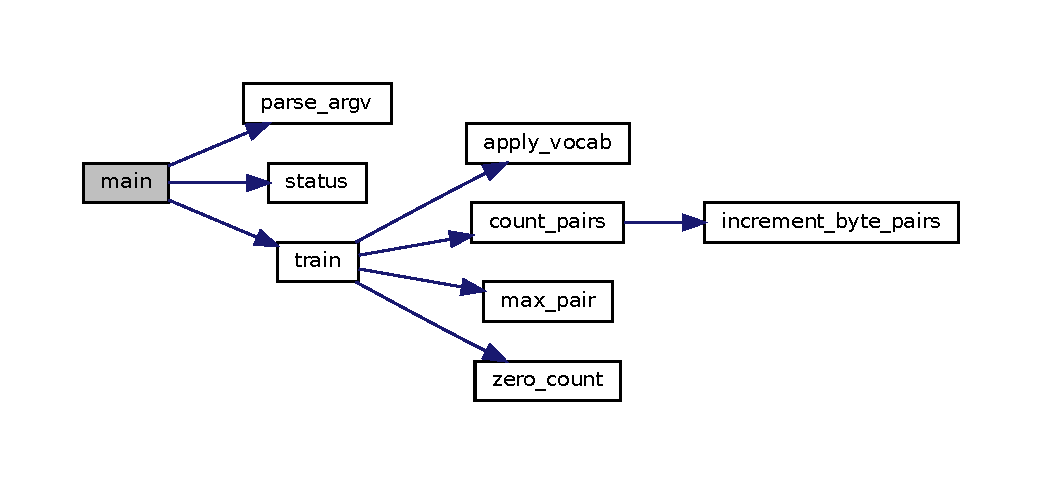
\includegraphics[width=0.6\textwidth]{original_application_callgraph.pdf}
    \caption{Call graph of the original application}
\end{figure}

The general algorithm of the original application is as follows

\begin{algorithm}[H]
    \caption{Original Application(mode, projectName, vocabSize, outputFilepath, inputFilepaths$[..N]$)} \label{alg:original}
    \textbackslash \textbackslash Input: String \textit{mode} which is either train or vocab, String \textit{projectName}, Natural number \textit{vocabSize}\\
    \textbackslash \textbackslash \hspace{1cm} String outputFilepath, many strings inputFilepaths that is \textit{N} long \\
    \textbackslash \textbackslash Output: File \textit{outputFilepath} with the vocabulary 
    \begin{algorithmic}[1]
        \State $vocabulary \gets \{\}$
        \If{mode == train}
            \For{$i\gets 0$}{$vocabLength$}
                \State $pairCounts \gets \{\}$
                \For{$j\gets 0$}{$N$}
                    \State $file \gets inputFilepaths[j]$
                    \State $buff \gets Read(file)$
                    \State $buff \gets transform(vocabulary, buff)$ 
                    \State $pairCounts \gets pairCounts \cup \text{countPairs}(buff)$
                \EndFor
                \State $vocabulary \gets vocabulary \cup \text{mostCommon}(pairCounts)$
                \State $outputFilepath \gets vocabulary$
            \EndFor
        \ElsIf{mode == status}
            \State $stdout \gets JSON(vocabulary)$
        \EndIf
    \end{algorithmic}
\end{algorithm}

If called with the command \mintinline{bash}{./train_vocab train project 260 output.vocab main.c} then the 
program will create a file called \textit{output.vocab} that contains the vocabulary of the files \textit{main.c}.
There will be a list of four replacements which are the most common byte pairs where each is recursively replaced from the 
start of the list. As main.c is a C file it will contain common pairs found in C source code. You can expect that the first replacement made 
will be $(32,32)$ to $256$ as $32$ is the ASCII code for a space character. If the author of the code
used four spaces for the indentation then the next most common pair will be $(256,256)$ which will be replaced with $257$.
 as the four 32's will have been replaced  with two 256's and then that will be replaced with a 257.


This vocabulary output can then be loaded at a later stage after being trained and used to encode 
some file you wish to feed into a language model.

A typical use case for this type of application is to take a large dataset, potentially multiple terrabytes of
data and use it to train a vocabulary so some statistical model can be fitted on the encoded data. 
This technique allows for the model to see a more uniform distribution of token values as performing
token level predictions on unencoded data would lead to it overfitting on the most common tokens.

\section{Potential Parallelism}
From the algorithm \ref{alg:original} it can be seen that how the vocabulary is used is a 
flow, output, and anti dependence with the loop from \textit{i} to \textit{vocabLength}. This is
because the vocabulary starts empty and is built up on each iteration, this requires the previous 
iteration's value to be available so the files can be correctly transformed, This is a flow dependence.
Then when the vocabulary is updated in each iteration it is an output dependence, and then in subsequent
iterations the vocabulary is used to transform the files which is later overwritten when it is updated, this is an anti dependence.

As the nature of the algorithm is to build up the vocabulary in a loop, it is not possible to parallelise the outer loop. 
This makes the inner loop the first candidate for parallelisation. The inner loop is a loop over the files that are to be trained on.
The original application is designed to preserve memory so on every iteration of the inner loop in algorithm \ref{alg:original} 
the file is read into memory, and then transformed. This makes sure it is in a state that matches the current point of training.
These files could be processed in parallel, this would give too rough of a granularity which is not desirable. 
If parallelising at the file level the program could have to wait on very large files to be processed 
in a serial manner. This would lead to poor utilisation of the available compute if the files are 
inbalanced in size regardless of the data to compute map.

Given the predicted poor load balance of the file level parallelism the operations the loop performs
were investigated. 

\subsection{Byte pair tokeniser transform}
To perform the tranformation there are two nested loops as per the following algorithm

\begin{algorithm}[H]
    \caption{Transform(vocabulary, buff)} \label{alg:transform}
    \textbackslash \textbackslash Input: Array of vocab \textit{vocabulary}, Array of symbols \textit{buff} \\
    \textbackslash \textbackslash Output: Array of symbols \textit{buff} with byte pairs replaced
    \begin{algorithmic}[1]
        \For{$i\gets 0$}{$len(vocabulary)$}
            \For{$j\gets 0$}{$len(buff)$}
                \If{$\text{buff}[i] == \text{SKIP\_TOKEN}$}
                    \State \textbf{continue}
                \EndIf
                \If{$\text{buff}[i] == \text{vocabulary}[j].b1$}
                    \State $p \gets 1$
                    \While{$j + p < len(buff)$}
                        \If{$\text{buff}[j+p] \neq \text{SKIP\_TOKEN}$}
                            \State \textbf{break}
                        \EndIf
                        \State $p \gets p + 1$
                    \EndWhile 
                    \If{$\text{buff}[i+1] == \text{vocabulary}[j].b2$}
                        \State $\text{buff}[i] \gets \text{vocabulary}[j].rep$
                        \State $\text{buff}[i+1] \gets \text{SKIP\_TOKEN}$
                    \EndIf
                    \State $j \gets j + p$
                \EndIf
            \EndFor
        \EndFor
    \end{algorithmic}    
\end{algorithm}

From the algorithm \ref{alg:transform} it can be seen that the inner loop and outer loops both have 
flow and anti dependences. This makes the algorithm unsuitable for parallelisation. This means for this algorithm applying
it to many files in parallel is the only suitable option.

\subsection{Counting byte pairs}

The algorithm for counting byte pairs is as follows

\begin{algorithm}[H]
    \caption{CountPairs(buff)} \label{alg:countpairs}
    \textbackslash \textbackslash Input: Array of symbols \textit{buff} \\
    \textbackslash \textbackslash Output: Array of array of numbers \textit{pairCounts}
    \begin{algorithmic}[1]
        \State $pairCounts \gets \{\}$
        \For{$i\gets 0$}{$len(buff)$}
            \If{$\text{buff}[i] == \text{SKIP\_TOKEN}$}
                \State \textbf{continue}
            \EndIf
            \State $p \gets 1$
            \While{$i + p < len(buff)$}
                \If{$\text{buff}[i+p] \neq \text{SKIP\_TOKEN}$}
                    \State \textbf{break}
                \EndIf
                \State $p \gets p + 1$ 
            \EndWhile
            \If{$i + p == len(buff)$}
                \State $\text{return} {}$
            \EndIf

            \State $b_1 \gets buff[i]$
            \State $b_2 \gets buff[i+p]$
            \State $pair[b_1][b_2] \gets pair[b_1][b_2] + 1$
        \EndFor
    \end{algorithmic}
\end{algorithm}

In the algorithm it can be seen that there is a flow and anti dependence in the loop.
As the only dependence is the pair array though it is classed as a reduction operation.
The reduction operation in this algorithm is non trivial as when indexing the pair there are 
possible branches and memory allocations that could be performed. This makes OpenMP's reduction clause
unsuitable for this operation. This would require a custom reduction operation to be implemented.

\subsection{The Clean Slate}

If the application is written from scratch and the parallelism available in the existing application is not
binding then through significant refactoring the application could be made to be more parallelisable.

\subsubsection{Dealing with data in chunks}
It was discussed earlier that the file level parallelism would be too rough of a granularity to be useful.
However if "files" were to be replaced with "chunks" then the granularity would be more fine grained. The chunk
can have a size that is controlled by the programmer and can be adjusted to suit the data being processed.

If the ghost cell pattern is used then the dependence on the byte prior to a chunk can be handled. The chunks can
also be created as a view to the original data so when the chunk is run through the transform the ghost cell 
pattern can be used to ensure that the chunk is transformed correctly. When creating the chunks the boundry must 
be checked to ensure that the chunk is not split in the middle of a byte pair that is to be replaced. 
This only works when one byte pair replacement transformation has to take place.


%Ghost cell pattern



\section{Mapping computation to processors}
OpenMP SIMD, and a manually managed thread pool created with POSIX pthreads

\section{Timing and profiling}

\section{Testing of logical equivalence}

\section{Tools used}

\section{Process and Problems encountered}

\section{Explaination of the code}

\section{Learnings}



\end{document}